\documentclass[12pt, twocolumn]{article}

\usepackage[utf8]{inputenc}
\usepackage[T1]{fontenc}
\usepackage{microtype}
\usepackage{fourier} 

\usepackage{amsmath, amssymb, amsthm}
\usepackage{mathtools} 

\usepackage[letterpaper, margin=1in, heightrounded]{geometry} 
\usepackage[skip=0.8em, indent=0pt]{parskip}
\usepackage{setspace}
\setstretch{1.15} 

\usepackage{tikz}
\usetikzlibrary{arrows.meta, calc, positioning, shapes.geometric}
\usepackage{pgfplots} 
\pgfplotsset{compat=1.18}

\usepackage{float} % <--- FIXED: Added this to resolve the [H] error

\newtheorem{theorem}{Theorem}[section]
\newtheorem{lemma}[theorem]{Lemma}
\newtheorem{proposition}[theorem]{Proposition}
\newtheorem{corollary}[theorem]{Corollary}

\theoremstyle{definition}
\newtheorem{definition}[theorem]{Definition}
\newtheorem{example}[theorem]{Example}

\theoremstyle{remark}
\newtheorem*{remark}{Remark}

% --- References & Links ---
\usepackage{xcolor}
\usepackage{hyperref}
\hypersetup{
    colorlinks=true,
    linkcolor=purple,  
    citecolor=blue,
    urlcolor=teal
}




\title{Trigonometry}
\author{Sarv Patel}
\date{\today}

\begin{document}

\maketitle
\section*{6.1 Radian Measure}

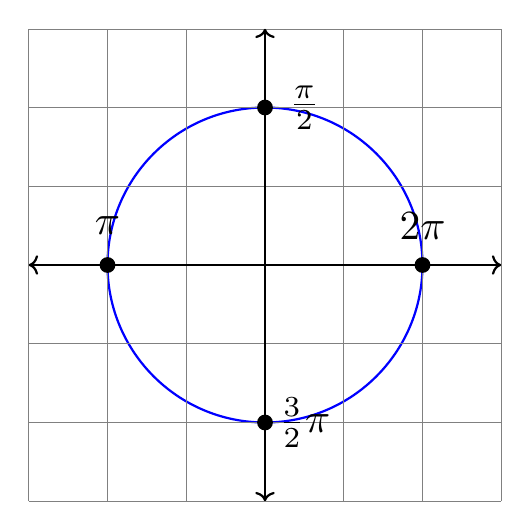
\begin{tikzpicture}
    \draw [blue,thick] (0,0) circle (2cm);
    \draw [step=1cm,gray,very thin] (-3,-3) grid (3,3);
    \draw [thick, <->] (0,3) -- (0,-3);
    \draw [thick, <->] (3,0) -- (-3,0);
    \node[scale=1.5] at (0.5,2) {$\frac{\pi}{2}$};
    \node[scale=1.5] at (2,0.5) {$2\pi $};
    \node[scale=1.5] at (-2,0.5) {$\pi $};
    \node[scale=1.5] at (0.5,-2) {$\frac{3}{2}\pi $};

  \fill (0,2) circle (0.1);
  \fill (2,0) circle (0.1);
  \fill (-2,0) circle (0.1);
  \fill (0,-2) circle (0.1);
\end{tikzpicture}


\end{document}





